\chapter{ClickNP编程平台介绍}
\section{系统架构}
ClickNP基于Catapult Shell体系结构搭建。该体系结构包含PCIe、直接内存访问(direct memory access, DMA)、
内存管理单元(memory management unit, MMU)、以太网介质访问控制(media access control, MAC)等
适用于多种应用场景的可服用逻辑,并将其抽象为定义好的接口。由ClickNP编写的FPGA程序生成的目标为Catapult功能。
由于ClickNP依赖的不同高级编程工具生成的目标接口不一致,因此在其下层有一个适配层,
将不同高级编程工具接口统一到Catapul Shell接口。

主机进程通过ClickNP库函数与FPGA程序通信,而库函数则依赖Catapult PCIe接口实现。
ClickNP库主要实现两个重要的功能:主机与FPGA之间的高速低延迟PCIe通道应用程序接口,
以及不同高级编程工具向FPGA模块传递参数并发送启动、停止、复位等信号的调用接口。

主机进程包括一个管理线程以及零个或多个工作线程。管理进程负责将程序镜像载入硬件、
启动工作进程、根据配置初始化FPGA和CPU中的ClickNP元件以及在运行时通过想各个元件发送信号来控制其行为。
在CPU的指派下,每个工作线程可以处理多个任务。

\section{程序设计}
\subsection{概念抽象}
ClickNP提供了模块化的编程模型,以元件为基本处理模块。每个元件包括以下属性:
\begin{description}
\item[本地状态]每个元件可定义一系列仅由自身访问的本地状态;
\item[输入输出端口]一个元件可以通过多个输入输出端口与其他元件通信;
\item[句柄函数]一个元件有三个句柄函数:初始化函数只在元件启动时执行一次;
处理函数在元件工作期间反复调用,处理输入的数据;信号函数类似于中断控制器,
在元件从主机进程收到信号时被调用,处理指令。
\end{description}

一个元件的输出端口可以用通道与另一个元件的输入端口连接。在ClickNP中,通道相当于一个先进先出的缓冲区,
从其一端写入,从另一端读取,如图~\ref{fig:channel}所示。
\begin{figure}
\centering
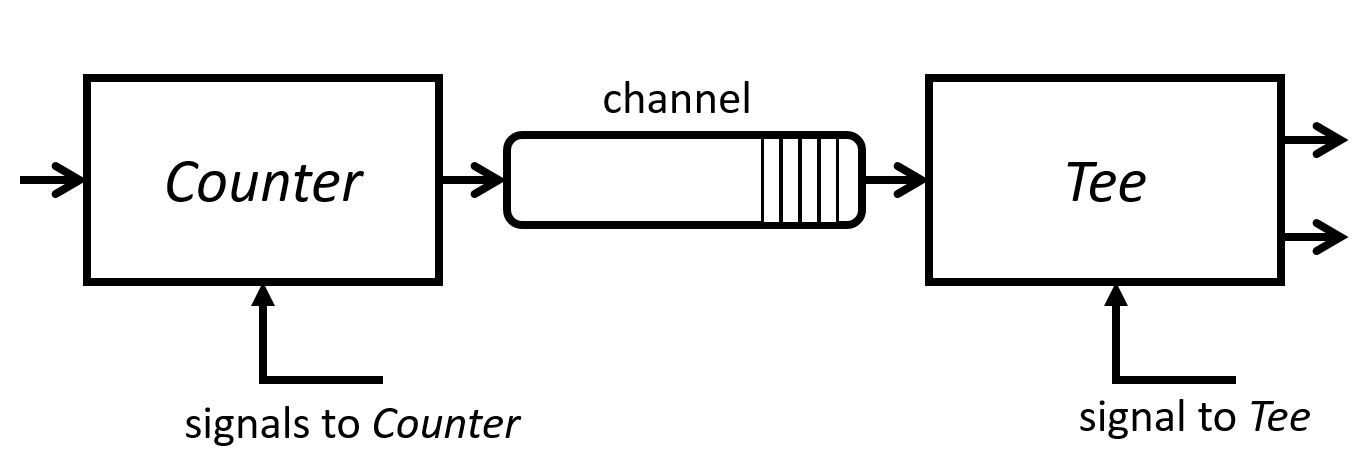
\includegraphics[width=4in]{channel}
\caption{通道} \label{fig:channel}
\end{figure}

每次通道读写操作的基本单位为帧,每个帧的大小固定为64字节,其中头部包含元数据,
数据载荷长32字节。如图~\ref{fig:flit}所示,其成员定义如下:
\lstinputlisting[language=C++]{code/flit.cl}

\begin{figure}
\centering
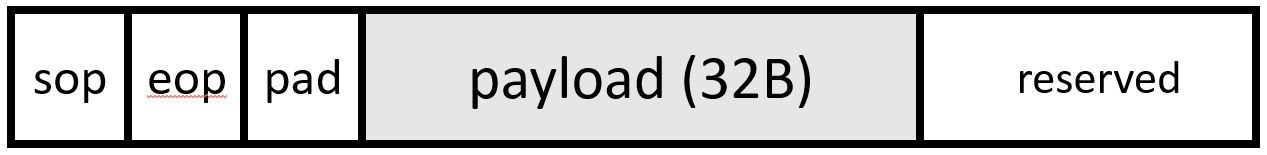
\includegraphics[width=4in]{flit}
\caption{帧} \label{fig:flit}
\end{figure}

以完整包为代表的大段数据会被拆分为多个帧在元件之间传播。其中第一帧的包开始位(start of packet, sop)置为真,
最后一帧的包结束位(end of packet, eop)置为真。如果数据载荷小于32字节,那么最后一帧的留白(padding, pad)域指代载荷的尾部留白区段大小。
将大的包拆分为帧,不仅能够降低延迟,还有助于提升处理包数据的各级流水线之间并行化程度。

在定义完各个元件之后,通过ClickNP配置文件将元件连接为有向图,使其互连,形成总的计算系统,
以下为一个远程直接内存访问(remote direct memory access, RDMA)处理器的配置文件,
其开头部分描述该系统依赖的元件类型,随后将元件实例化,并用箭头表示其通道连接关系。
\lstinputlisting{code/RoCE.cfg}
